\chapter{The CloudyPeer framework}
As is stated in the
introduction, \cloudypeer aims to be a general framework for building
\ptop application focused on data dissemination scenarios.
In particular the final goal of the project is to give developers the
ability to create such applications with the minimum amount of code as
possible, concentrating their effort in planning the logic of the
application instead of the underlying \ptop infrastructure.

This convenience however must not come at the price of
flexibility: often times the design of a \ptop application requires
tweaking at the lower level of the infrastructure; in these situations
a static and monolithic framework may represent an obstacle instead of
an help.
In this regards \cloudypeer must enable developers to extend its
functionality in an easy and integrated way without breaking the other
requirements.

Another important factor which has been considered during the
planning phase is that the performances of a \ptop application may
vary substantially by changing the specific protocol offering a
particular functionality, or by tuning its parameters. Often this
evaluation stage is performed in a simulated environment due to timing
constraints and ease of development. However simulations not always
reflect what happens when the same protocol is implanted in a real
scenario.
The \cloudypeer architecture has been explicitly designed to allow the change
of every single component by simply modifying a configuration
parameter thus allowing experimenting with different
combinations without the need to touch a single line of code.

The implementation is based on the \emph{Java} programming language
and it is compatible with version 1.5 or higher. The
choice of \emph{Java} is motivated by the fact that it provides a rich
\emph{standard library} and its object oriented nature makes it a
perfect candidate for designing an extensible framework. Furthermore
the existence of many commercial and open-source projects written in
\emph{Java} and concerning \ptop systems represent a valuable resource
in term of code reuse.
\ \\
In the following sections will be analyzed the architecture of
\cloudypeer by describing it is major components and their interactions.
Furthermore will be described the various module's
built-in implementations and the means offered to developers to extend
the framework itself.
In conclusion a ``toy'' application will be shown with the intent of
demonstrating the simplicity and the convenience offered by
\cloudypeer.

As for the previous chapter the notation rules adopted in the
following portion of the chapter are:
\begin{itemize}
  \item serif font for files and directories, i.e. \textsf{ExampleFile.java},
    \textsf{./example\_directory/}
  \item italics font with capitalized initials for module names,
    i.e. \textit{Example Module}
 \item typewriter font for class names, i.e. \texttt{ExampleClass}
  \item italics font followed by parenthesis for methods
    i.e. \textit{exampleMethod()}
  \item standard UML notation for diagrams
\end{itemize}

\section{Architecture}
Figure \ref{fig:cloudypeer-architecture} shows an overview of the
architecture of \cloudypeer illustrating the principal components and
the way they are related one another.

\begin{figure}[h!]
  \centering
  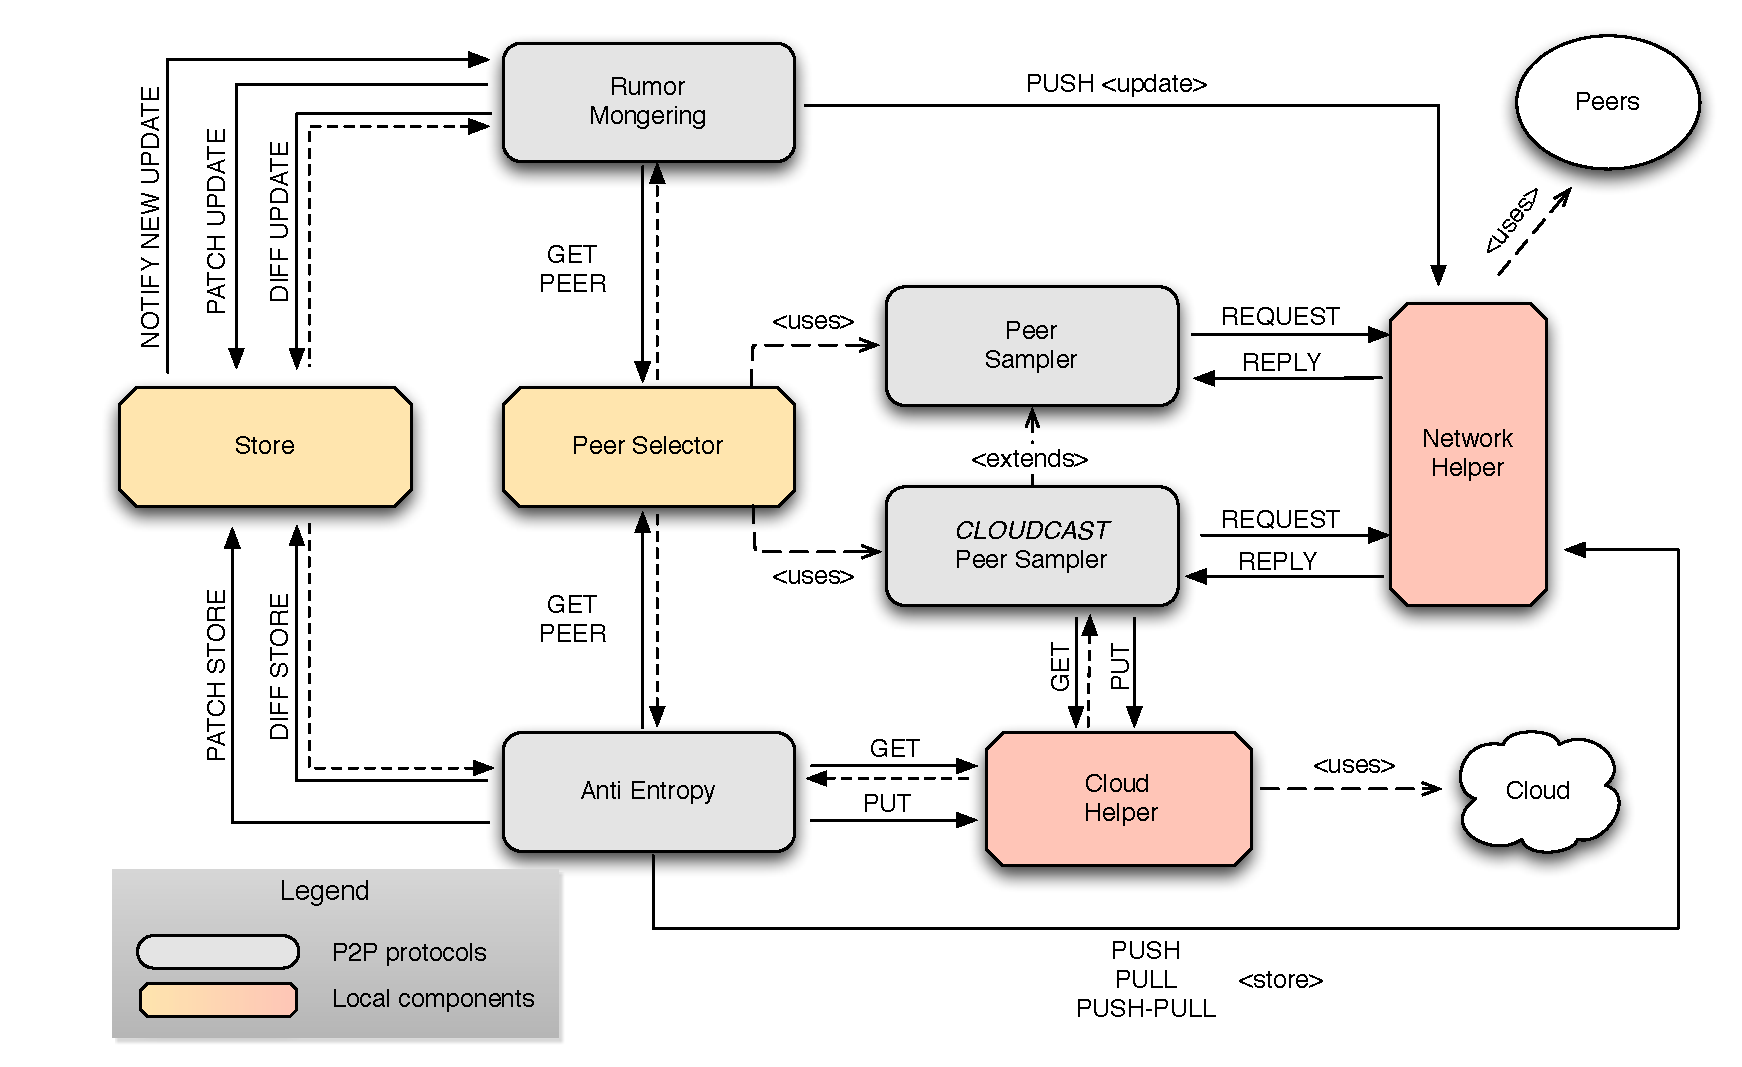
\includegraphics[width=\textwidth]{cloudypeer-architecture.pdf}
  \caption{Architectural overview of \cloudypeer}
  \label{fig:cloudypeer-architecture}
\end{figure}

As can be seen, the \peersampling protocols hold a central role in the
infrastructure and are divided in two categories: the first represents
classic protocols such as \cyclon; the second extends the former and
embodies the \peersampling protocol of \cloudcast.

Samples of the network's partial \view\ are offered to higher level
protocols via a \peerselector. This is a local module which does not
directly interact with the \ptop network but it just implements the logic
used by the application to select peers. This abstraction gives the
opportunity to application's developers to implement complex selection
strategies, possibly involving multiple \peersampling instances of
different kind. A simple implementation performing a random
selection with customizable filters is provided within the framework
and should be sufficient for most of the simpler scenarios.

The \peerselector itself is used by all the algorithms which are
based on the interaction between pairs of peers. At the current stage
the only components of such kind are the two variants of \epidemic
broadcast, but more can be easily added.

The function executed by these two protocols necessarily requires
access to the application data. However such a direct dependency
does not fit with
the generality requirement of the framework. For this reason the
\store abstraction layer has been added: this component provides a general
\api for accessing and managing the application's data exploitable by
other modules.
Application designers must create their own \store implementation
reflecting their storage model. To simplify this task the framework
provides a built-in implementation which takes care of most of the
operation needed to fulfill the \api specifications.

The modules which conclude this architecture overview are the
\cloudhelper and \networkhelper: similarly as what has been discussed for
\grapes, these two elements provide an abstraction layer which hides
the details of the actual implementations making it possible
to easily switch \cloud provider or networking technique.

\ \\
The following sections will cover the details of the aforementioned
modules by providing a more in depth description of the \api they
offer and by giving some insight on the way to extend them.

\section{Basic components}
Before starting the description about the specific modules, let's look
at figure~\ref{fig:cloudypeer-basic-relations} where are shown the
basic components which are used by the rest of the \cloudypeer
infrastructure.

\begin{figure}[h!]
  \centering
  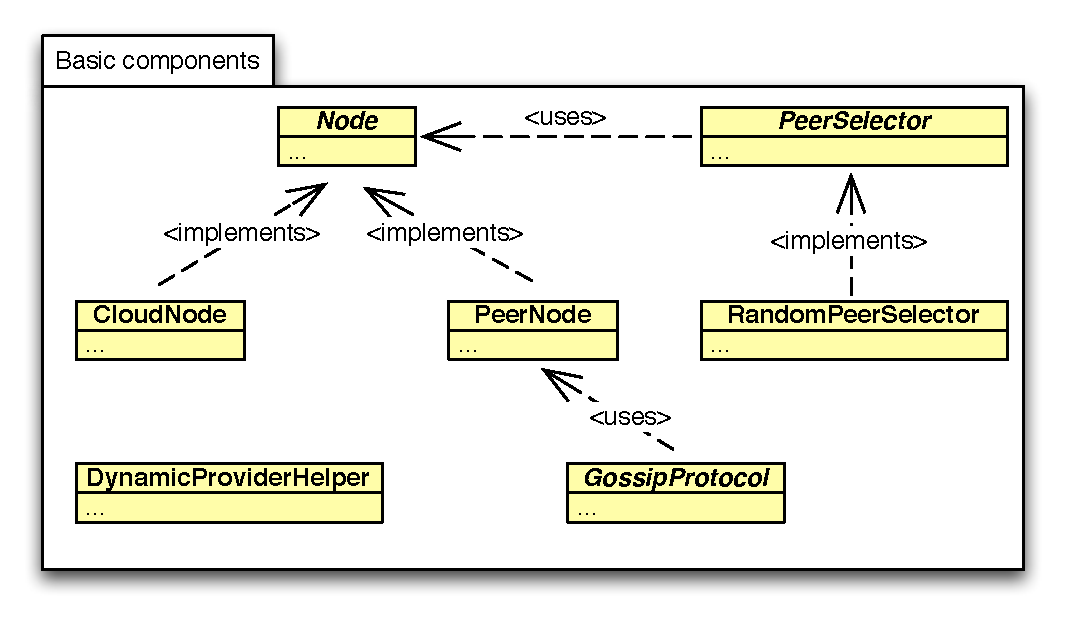
\includegraphics[width=\textwidth]{cloudypeer-basic-relations.pdf}
  \caption{\cloudypeer basic components}
  \label{fig:cloudypeer-basic-relations}
\end{figure}

Most of the classes role should be already clear at this point:
\texttt{Node} and its two implementation are used to model
node \descriptors and provide basic addressing information while
\texttt{PeerSelector} defines a standard way to express
peer selection strategies, of which \texttt{RandomPeerSelector} is a
simple example.

The remaining two classes instead deserve more attention.
\texttt{DynamicProviderHelper} is an utility component which
provides the infrastructure needed to dynamically load object's
implementations. It performs a hierarchical parsing of provider's
configurations file, enabling end-user to overwrite the built-in
values, and handles the instantiation of the correct
implementation via name mappings. Since its presence results completely
transparent to users of \cloudypeer, it is not proposed a detailed
description. Developers interested in extending the
framework with new protocols may refer to the \javadoc of the project
for further information on how to exploit the dynamic loading procedures.

\begin{figure}[h!]
  \centering
  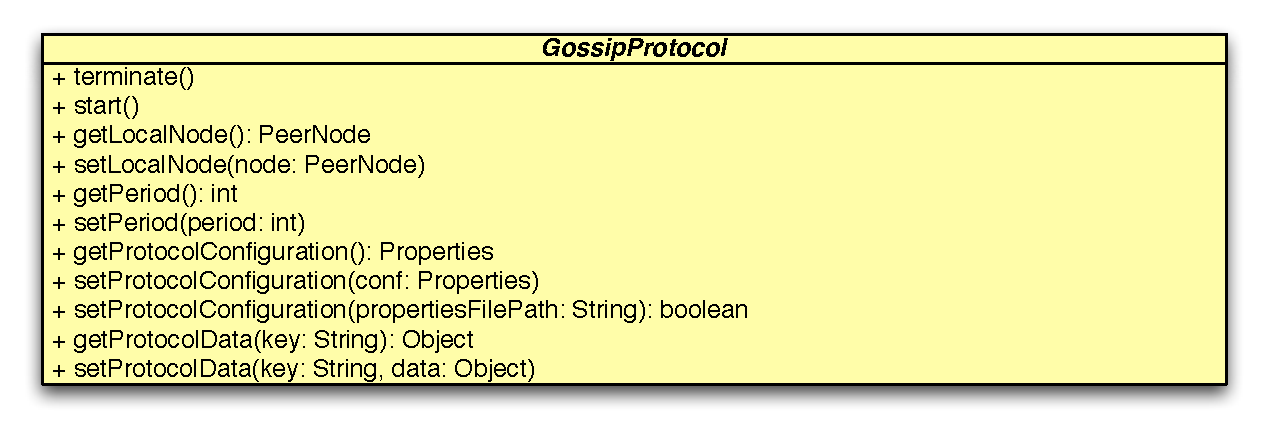
\includegraphics[width=\textwidth]{cloudypeer-basic-gossipprotocol-classdiagram.pdf}
  \caption{\texttt{GossipProtocol} public \api}
  \label{fig:cloudypeer-gossipprotocol-class}
\end{figure}

The last class composing the basic infrastructure is
\texttt{GossipProtocol}. A diagram describing this abstract class is
provided in figure~\ref{fig:cloudypeer-gossipprotocol-class}. This
component defines the skeleton of a \gossip protocol: it provides
standard means to start and stop the execution, configures the common
properties and furthermore it offers support for opaque parameters
and resources. Such features represent the public \api and
only reflect part of the offered functionalities: indeed
\texttt{GossipProtocol} implements many other common procedure aimed at
simplifying the thread management and the overall life-cycle of the
implementation.

\section{\networkhelper}
The \networkhelper module mission is to provide a simple abstraction
layer to the actual networking implementation. Its services are
available to any class wanting to use them, however its usage is not
required to build a protocol in \cloudypeer. Its design is somewhat
inspired to the relative component of \grapes, but with some
additional features.

\begin{figure}[h!]
  \centering
  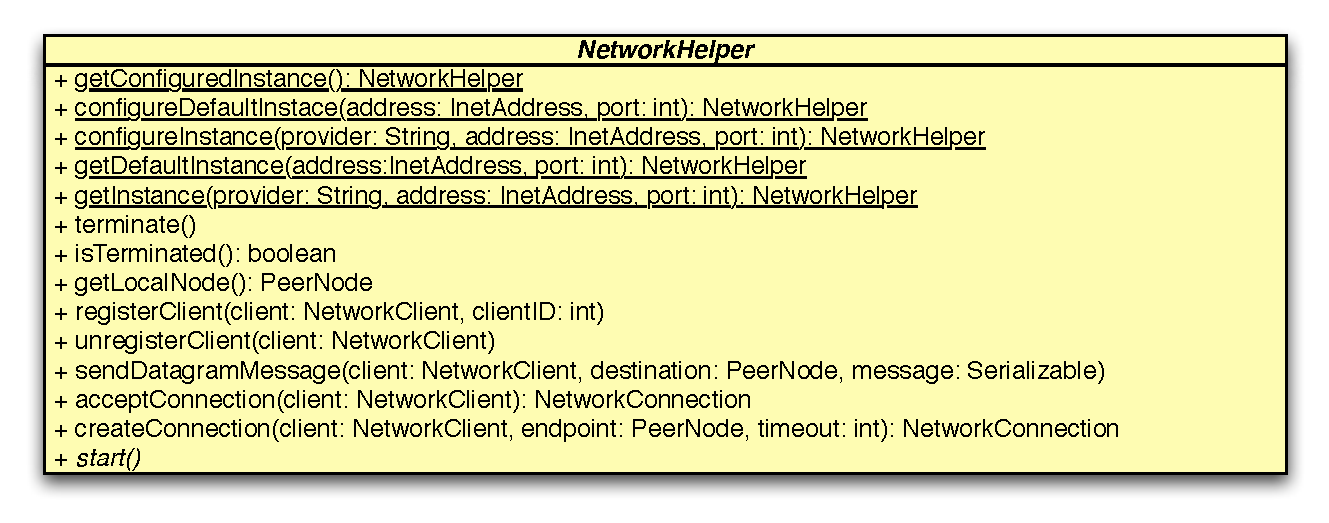
\includegraphics[width=\textwidth]{cloudypeer-networkhelper-classdiagram.pdf}
  \caption{\texttt{NetworkHelper} public \api}
  \label{fig:cloudypeer-nethelper-class}
\end{figure}

As can be seen by looking at the public \api shown in
figure~\ref{fig:cloudypeer-nethelper-class}, beyond datagram messages
\cloudypeer's \networkhelper offers support for connection oriented
transport protocols. The rationale of this choice resides in the fact
that some \ptop protocols require the exchange of a series of messages
to complete a cycle. Even though such requirement may be efficiently
achieved only by using datagram messages, the resulting code complexity is
substantial: by delegating this task to the \networkhelper, protocols
implementation can be much simpler. Even better, this strategy allow
for far more effective code re-usage: custom connection schemes can be
implemented as a \networkhelper object and made available to
all \cloudypeer component by simply changing a configuration parameter.

\begin{figure}[h!]
  \centering
  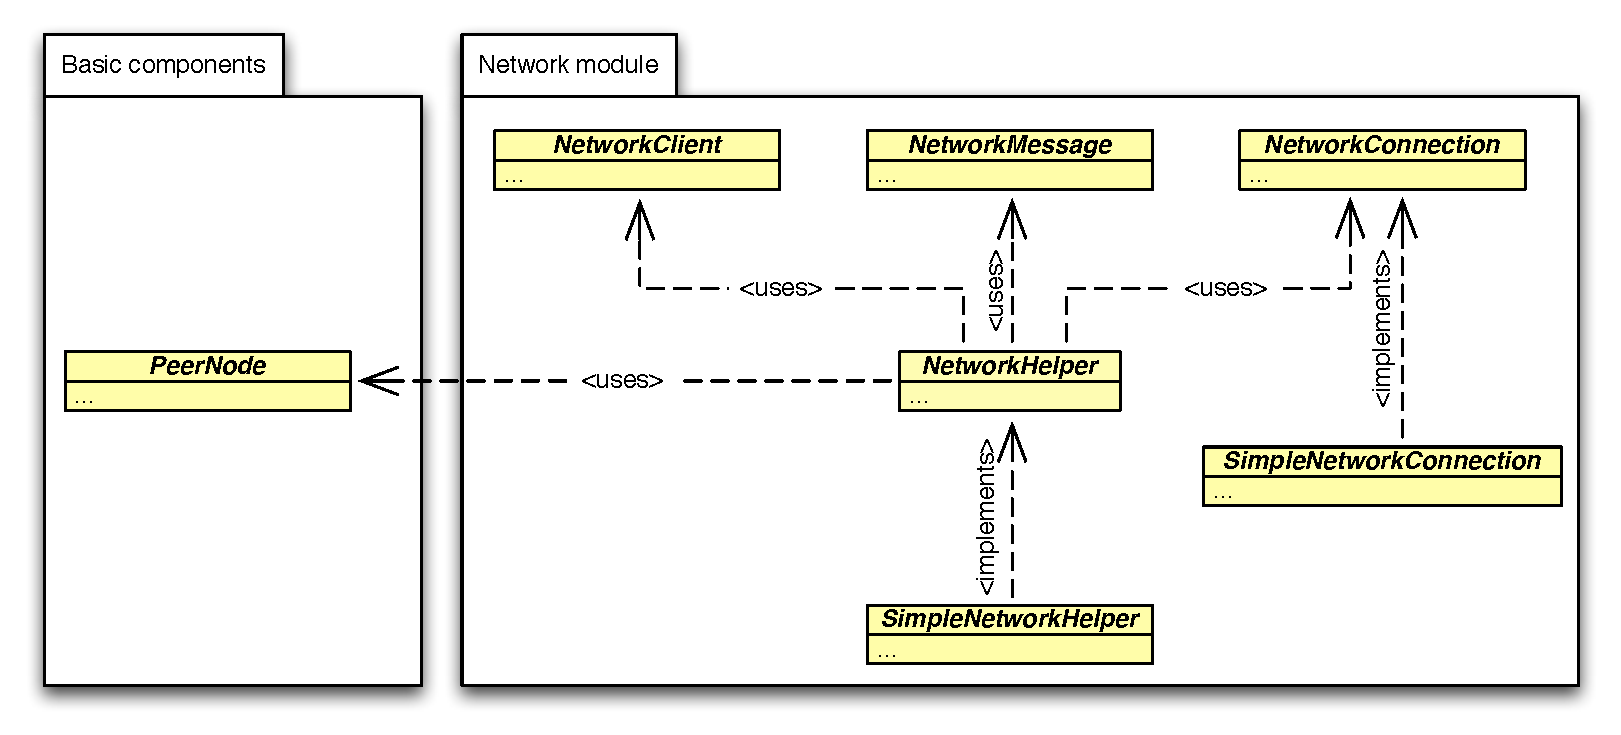
\includegraphics[width=\textwidth]{cloudypeer-networkhelper-relations.pdf}
  \caption{Relations between classes of the \networkhelper module}
  \label{fig:cloudypeer-nethelper-relations}
\end{figure}

A \networkhelper instance can be initialized by calling either the
\textit{getDefaultInstance()} or \textit{getInstance()} methods. The former
will load the default implementation as specified in the bundled
configuration file. The latter allows the caller to specify the
implementation to use. Another way to create a \networkhelper instance
is to ``configure'' it via the \textit{configureDefaultInstance()} or
\textit{configureInstance()} methods. In this way the newly created
instance will be stored and can be the recovered calling the
\textit{getConfiguredInstance()} method.

Before a class is allowed to exploit a \networkhelper instance it must
implement the \texttt{NetworkClient} interface and
``register'' itself by calling \textit{registerClient()}. The
registration phase maps the actual client instance to a specified
identifier. At this point the class can send datagram messages or
initiate connections to its remote counterparts. This means that a
\texttt{NetworkClient} can communicate only with remote
\texttt{NetworkClient} instances sharing the same identifier.

\ \\
At the current stage only one \networkhelper implementation is
distributed with the framework: \texttt{SimpleNetworkHelper}. This class
relays on \emph{Java}'s network stack and exploits threads to allow
concurrent connections. In particular connection oriented
communication is achieved via the \texttt{TCP} protocol.
Another implementation, which has not been completed due to time
constraints, is based upon \grapes's \networkhelper thus inheriting
the \emph{NAT traversal} supports.

\section{\cloudhelper}
The support for the \cloud storage service is offered via the
\cloudhelper module. Figure~\ref{fig:cloudypeer-cloudhelper-relations}
shows the components belonging to the module and their relations.
The central entity is \texttt{StorageCloud} which
implements the actual \cloud interaction logic. The offered \api, reported
in figure~\ref{fig:cloudypeer-cloudhelper-class}, deals with the
common operation supported by the various storage services. The
methods themselves are self-explanatory and should not require further
discussion.

A side note is however deserved by \texttt{CloudURI}: this
class provides a standard way to identify resources residing on the
\cloud. As can be seen by the \texttt{StorageCloud} diagram, an
instance of this class is required for the initialization phase to
identify the \textit{bucket} on which operate. Given that different
\cloud services may adopt profoundly different addressing schemes,
each \cloudhelper provider employs its own version of
\texttt{CloudURI} which applications obtain via the usual dynamic
loading strategy.

\begin{figure}[h!]
  \centering
  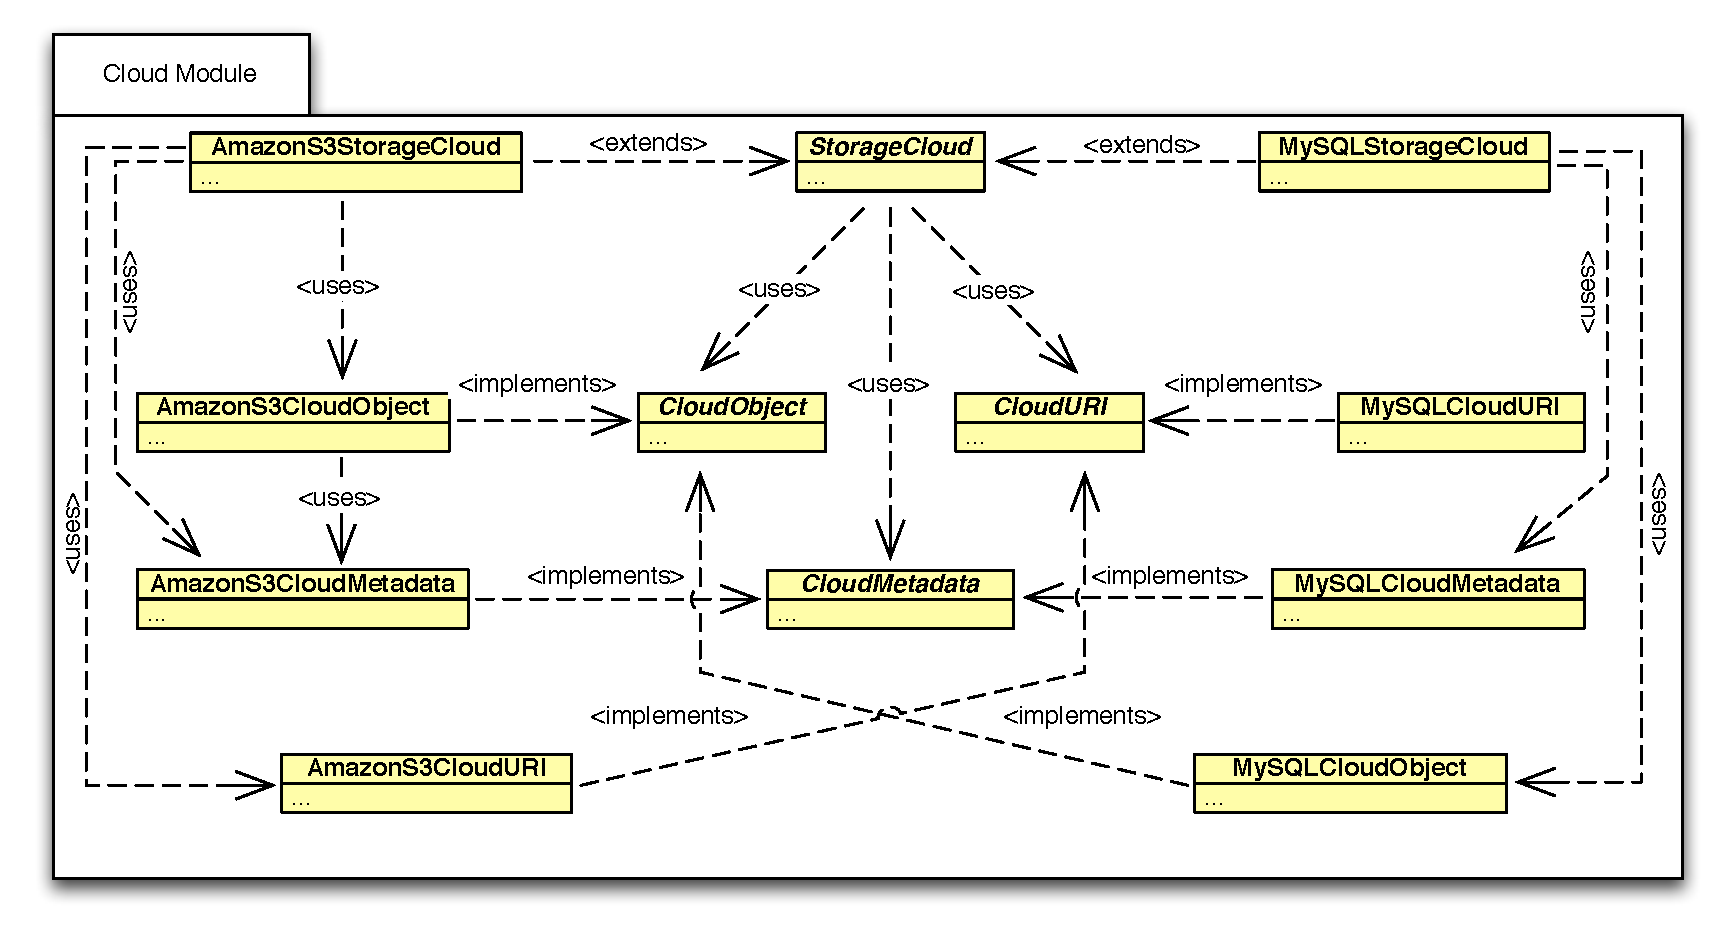
\includegraphics[width=\textwidth]{cloudypeer-cloudhelper-relations.pdf}
  \caption{Relations between classes of the \cloudhelper module}
  \label{fig:cloudypeer-cloudhelper-relations}
\end{figure}

\begin{figure}[h!]
  \centering
  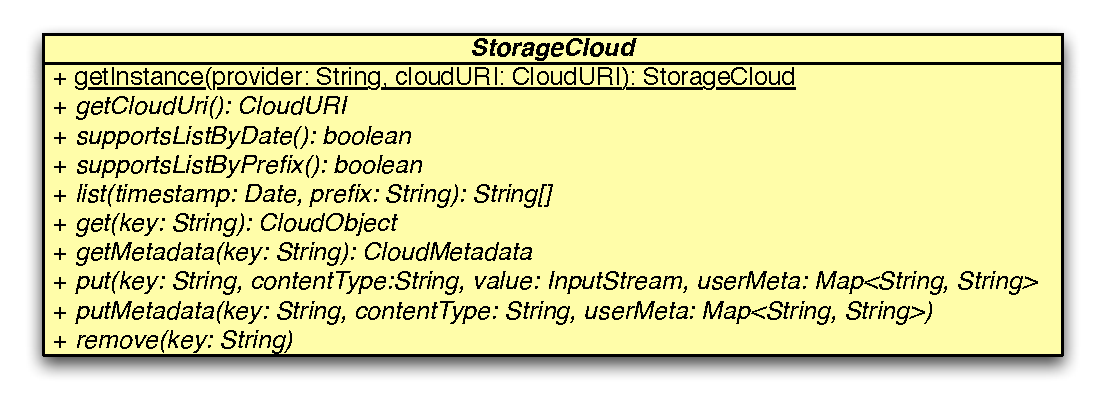
\includegraphics[width=\textwidth]{cloudypeer-cloudhelper-classdiagram.pdf}
  \caption{\texttt{StorageCloud} public \api}
  \label{fig:cloudypeer-cloudhelper-class}
\end{figure}

\ \\
The framework distribution ships two built-in \cloudhelper implementation
respectively for \textit{Amazon Simple Storage Service} and a
\textit{MySQL} backed \cloud service. The former is built upon
the official \textit{Amazon AWS SDK for Java}~\cite{AWS4Java} and it is
configured under the ``amazons3'' provider name, the latter
exploits the \textit{MySQL Connector/J}~\cite{MySQLConnectorJava} and
it is made available via the the ``mysql'' provider name.

The \textit{MySQL} \cloud is compatible with the one supported by
\grapes hence allowing the use of the same instance for both the
\peersampling and the actual storage. Table~\ref{tbl:mysql-cloud}
shows the base schema which a table must adhere to in order to being
used as a \cloud.

\begin{table}[H]
  \centering
  \begin{tabular}{|l|l|}
  \hline
  Field & Type \\
  \hline
  \hline
  cloud\_key & VARCHAR PRIMARY KEY \\
  cloud\_value & BLOB \\
  cloud\_timestamp &  INT UNSIGNED \\
  cloud\_content\_md5 &  VARCHAR(32) \\
  cloud\_content\_length &  INT UNSIGNED \\
  cloud\_content\_type & VARCHAR \\
  counter & INT UNSIGNED \\
  \hline
  \end{tabular}
  \caption{Schema of a \cloud enabled \textit{MySQL} table}
  \label{tbl:mysql-cloud}
\end{table}

\section{\textit{Store} module}
This module represents a key component of the \cloudypeer architecture
as it is responsible for all the storage-related tasks. As can be seen
by the extensive \api, shown in figure
\ref{fig:cloudypeer-store-class}, such operations range from simple
listing and management duties to much more complex procedures aimed at
efficiently resolving differences between instances.

\begin{figure}[h!]
  \centering
  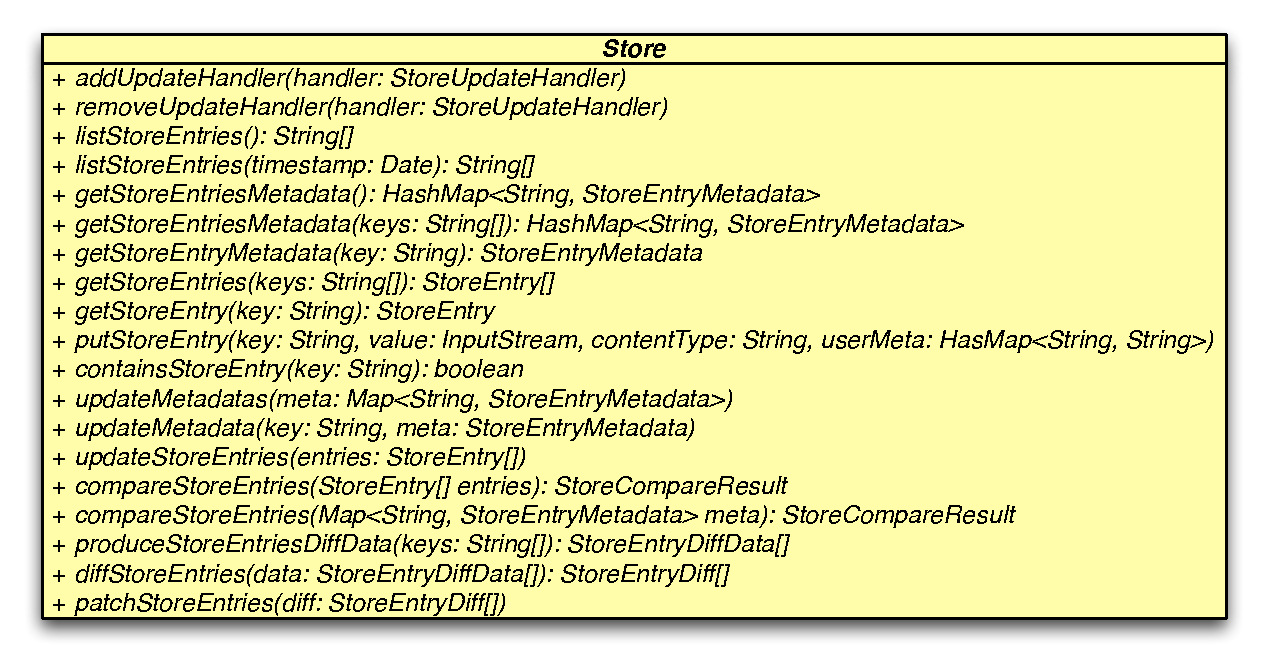
\includegraphics[width=\textwidth]{cloudypeer-store-classdiagram.pdf}
  \caption{\texttt{Store} public \api}
  \label{fig:cloudypeer-store-class}
\end{figure}

The former kind of operations are quite intuitive and for the most
part should not require additional comments. The only noteworthy
detail is that the version of \textit{listEntries()} without parameters
has a peculiar behavior: the returned values may represent only a
partial view of the entire entries: specifically the ``active''
portion. The definition of ``active'' is application dependent and
expresses some innate property of the domain. For instance in a news
distribution scenario it may be based on time constraint as it is likely
that users are not interested in news which are too old.

Shifting the focus to the more complex operations, let's look at the
two variants of
\textit{compareStoreEntries()}: these methods compare the \texttt{Store}
state against an array of entries and compile a report which specifies
two entries' set. The first contains all the entries
which are \textit{fresher} on the local instance while the second embodies
the ones that should be updated due to being old or unknown.

Such information is of major importance to resolve the differences between
\texttt{Store} instances: this can be done either by replacing the old
entry with the fresher one or by updating only the portion of data
 which is changed. The second method is based on the
concept of \textit{diff} and \textit{patch}: the two entries are
compared and the list of their differences is computed (diff),
subsequently the oldest entry is updated by replaying the listed
modification (patch).

Remembering that we are working in a \ptop scenario an immediate
problem arises: we cannot transfer the whole entry to perform the
diff or this would nullify the purpose of the procedure. Similarly
we cannot maintain a record of all the remote instances states to
locally compute differences, as the
\ptop nature of the system would quickly render such records outdated
and thus useless. The only
viable approach is for the source \texttt{Store} to produce some data
which enables the remote instance to compute the differences.

For example a simple strategy is to divide the data in chunks and
compute an hash value for each of them. Once a remote instance receives
the list of hashes, it can compute its hashes and then
compare the two results. An even better approach would be to use some
\textit{rolling  checksum}~\cite{Rsync} scheme.
The \api enables this line of action via the methods:
\textit{produceStoreEntriesDiffData()}, \textit{diffStoreEntries()} and
\textit{patchStoreEntries()}.

The last feature provided by the \textit{Store} module is represented
by the interface \texttt{StoreUpdateHandler} which allows the event
driven notification of storage changes.

\begin{figure}[h!]
  \centering
  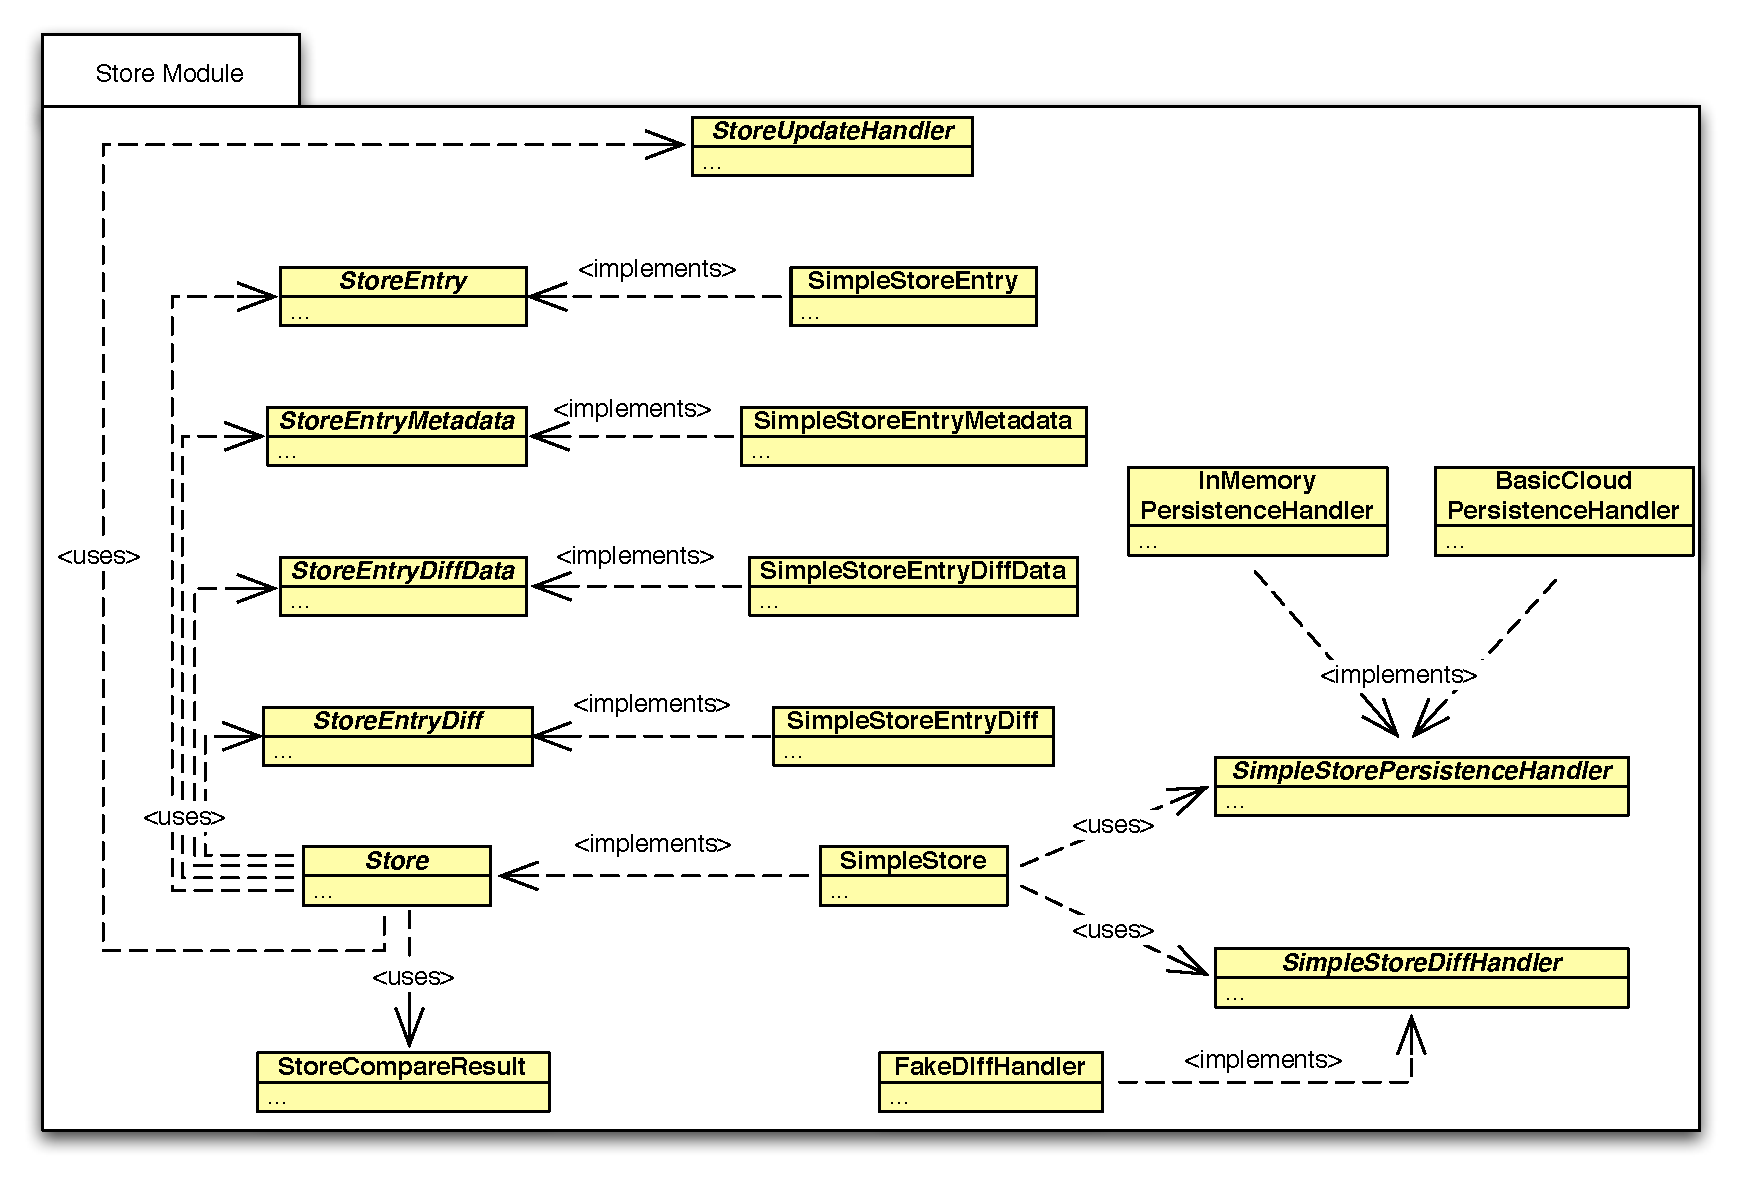
\includegraphics[width=\textwidth]{cloudypeer-store-relations.pdf}
  \caption{Relations between classes of the \cloudhelper module}
  \label{fig:cloudypeer-store-relations}
\end{figure}

\ \\
As shown in the module overview proposed in
figure~\ref{fig:cloudypeer-store-relations} the framework is
distributed with a built-in \texttt{Store} implementation providing
most of the basic functionalities, delegating only the management of the
actual persistence and \textit{diff} strategy. Developers can design their
own persistence layer by subclassing
\texttt{Simple\-Store\-Persistence\-Class} and developing \textit{write}, \textit{read} and
\textit{list} procedures. Two default implementations of this class are
made available: the first exploits the \cloudhelper to use a \cloud
instance as storage, the second instead keeps all its entries in
memory and is intended as a local storage implementation.

Similarly, different \textit{diff} schemes can be implemented by
extending \texttt{Simple\-Store\-Diff\-Handler} and writing
an implementation of the three action describes above. Given that
these are strictly dependent on the application scenario, the
framework only ships with a \textit{fake} component which makes the
\texttt{Store} compatible with protocols exploiting this
functionality, relaying however on the transmission of the complete data.

\section{\emph{Peer sampling} protocols}
All the components which are employed by \cloudypeer to provide
support for \peersampling protocols are enclosed in a module called
\textit{Peer Sampling}. The diagram of the various classes and their
relations is proposed in figure~\ref{fig:cloudypeer-peersampling-relations}.

\begin{figure}[h!]
  \centering
  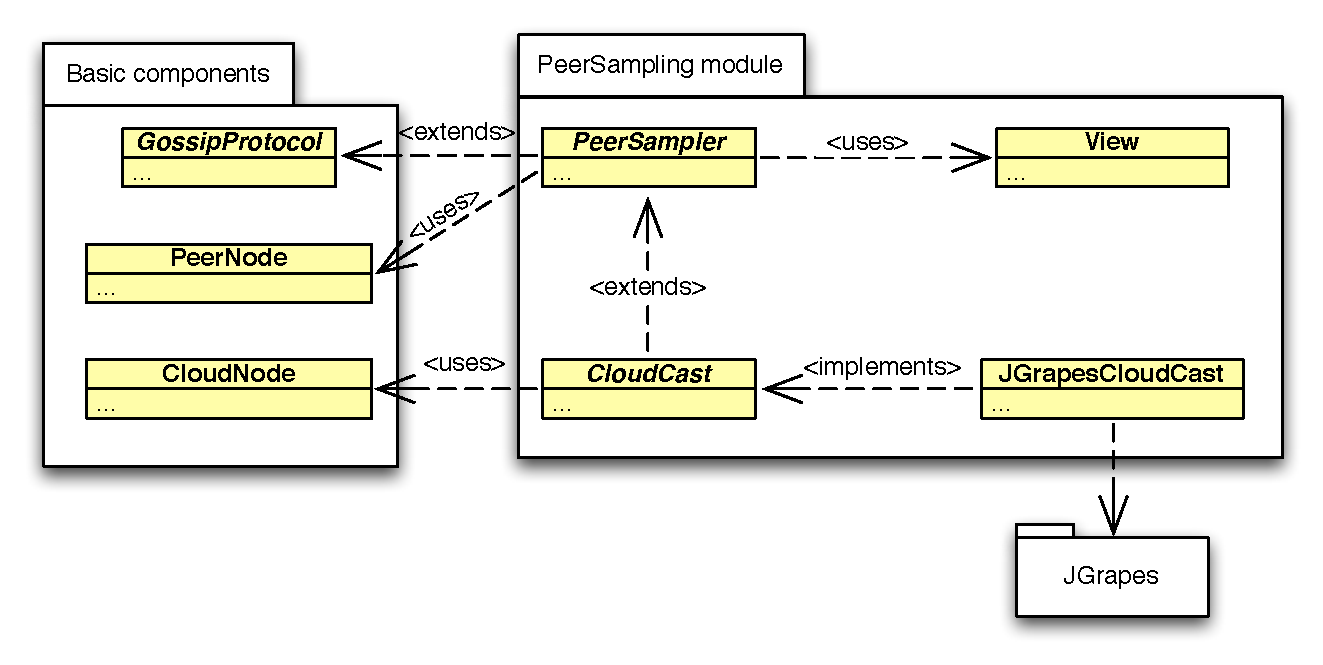
\includegraphics[width=\textwidth]{cloudypeer-peersampling-relations.pdf}
  \caption{Relations between classes of the \peersampling module}
  \label{fig:cloudypeer-peersampling-relations}
\end{figure}

Given that this work has been mainly concerned with implementing a
\cloudcast based application, the only available protocol at this time
is represented by \texttt{CloudCast}. However support for
conventional protocols can be added simply by subclassing
\texttt{PeerSampler}. The task if further simplified by the fact that
\grapes already implements some of them, hence it is sufficient to
write a wrapper which just performs the data conversion and delegates
all the real work to the library. Indeed this very strategy is adopted
by the built-in \texttt{JGrapesCloudCast} implementation.

The \api provided to developers can be seen in the diagram proposed in
figure~\ref{fig:cloudypeer-peersampling-class}. All the basic
functionalities are inherited by \texttt{GossipProtocol}, hence the
\texttt{PeerSampler} only need to define the standard methods to
interact with the network partial \view. As can be seen by looking at
the \texttt{CloudCast} definition, all that is left for the actual
protocol classes to specify is the instantiation mechanism and
possibly methods to manage additional parameters.

\begin{figure}[h!]
  \hspace{-50pt}
  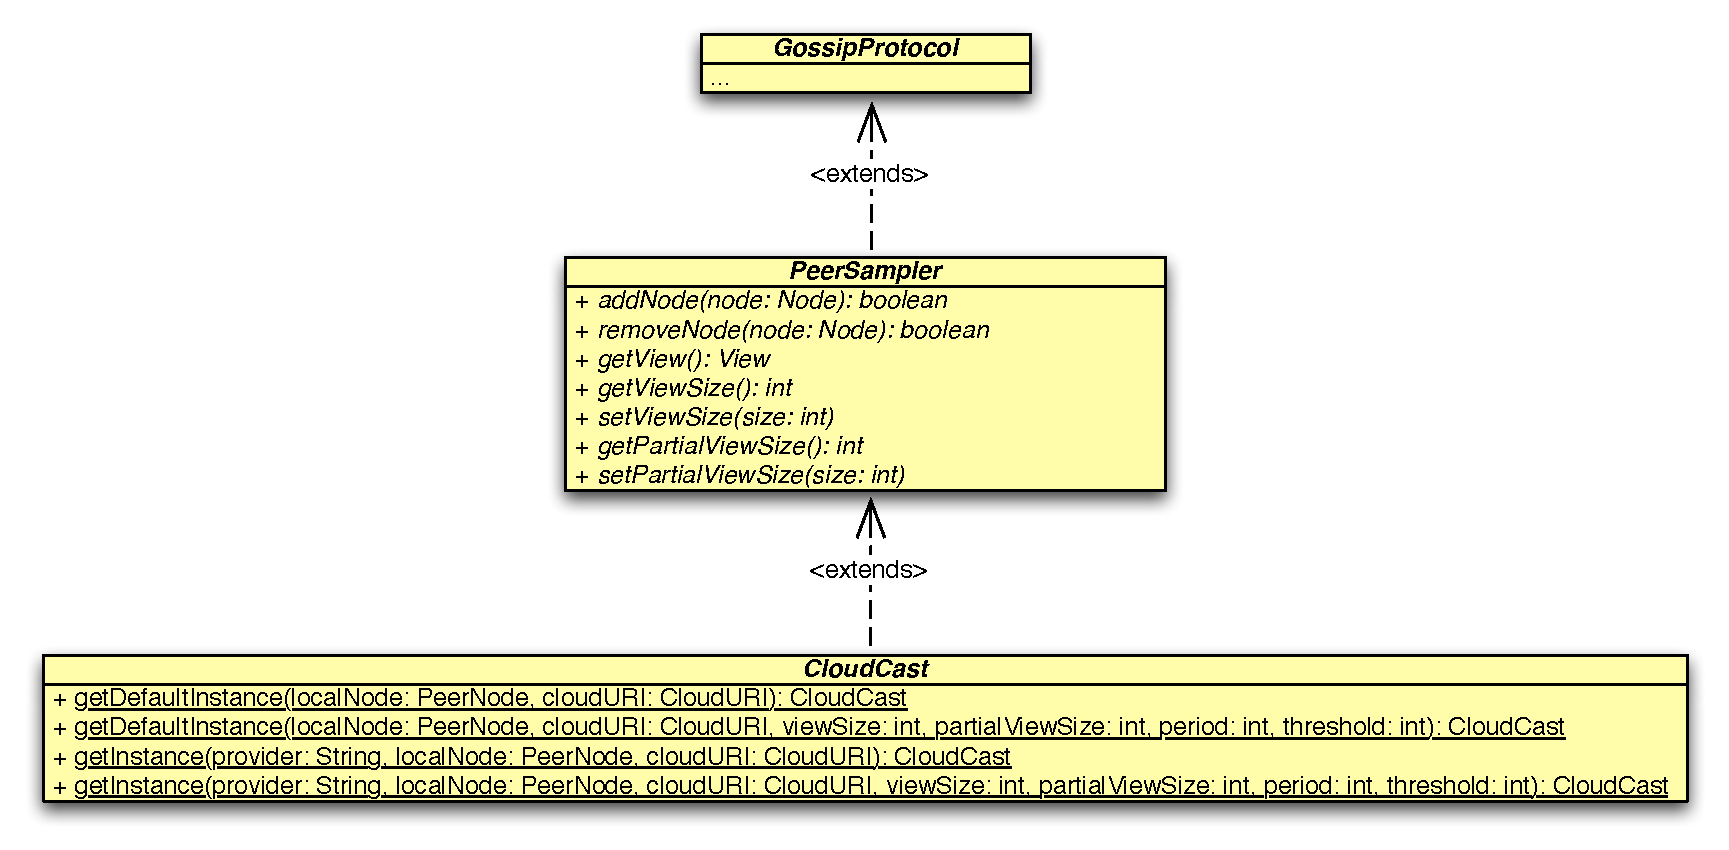
\includegraphics[width=1.3\textwidth]{cloudypeer-peersampling-classdiagram.pdf}
  \caption{Details of the \texttt{CloudCast} \api}
  \label{fig:cloudypeer-peersampling-class}
\end{figure}

The offered \api is simple enough that a detailed description is not
appropriate in this context. More information on the meaning of the
various parameters can be found in the \javadoc of the various
classes.

\section{\emph{Epidemic broadcast} protocols}
The module that concludes this overview of the \cloudypeer
architecture is the one providing the infrastructure for the \epidemic
protocols.

\begin{figure}[h!]
  \centering
  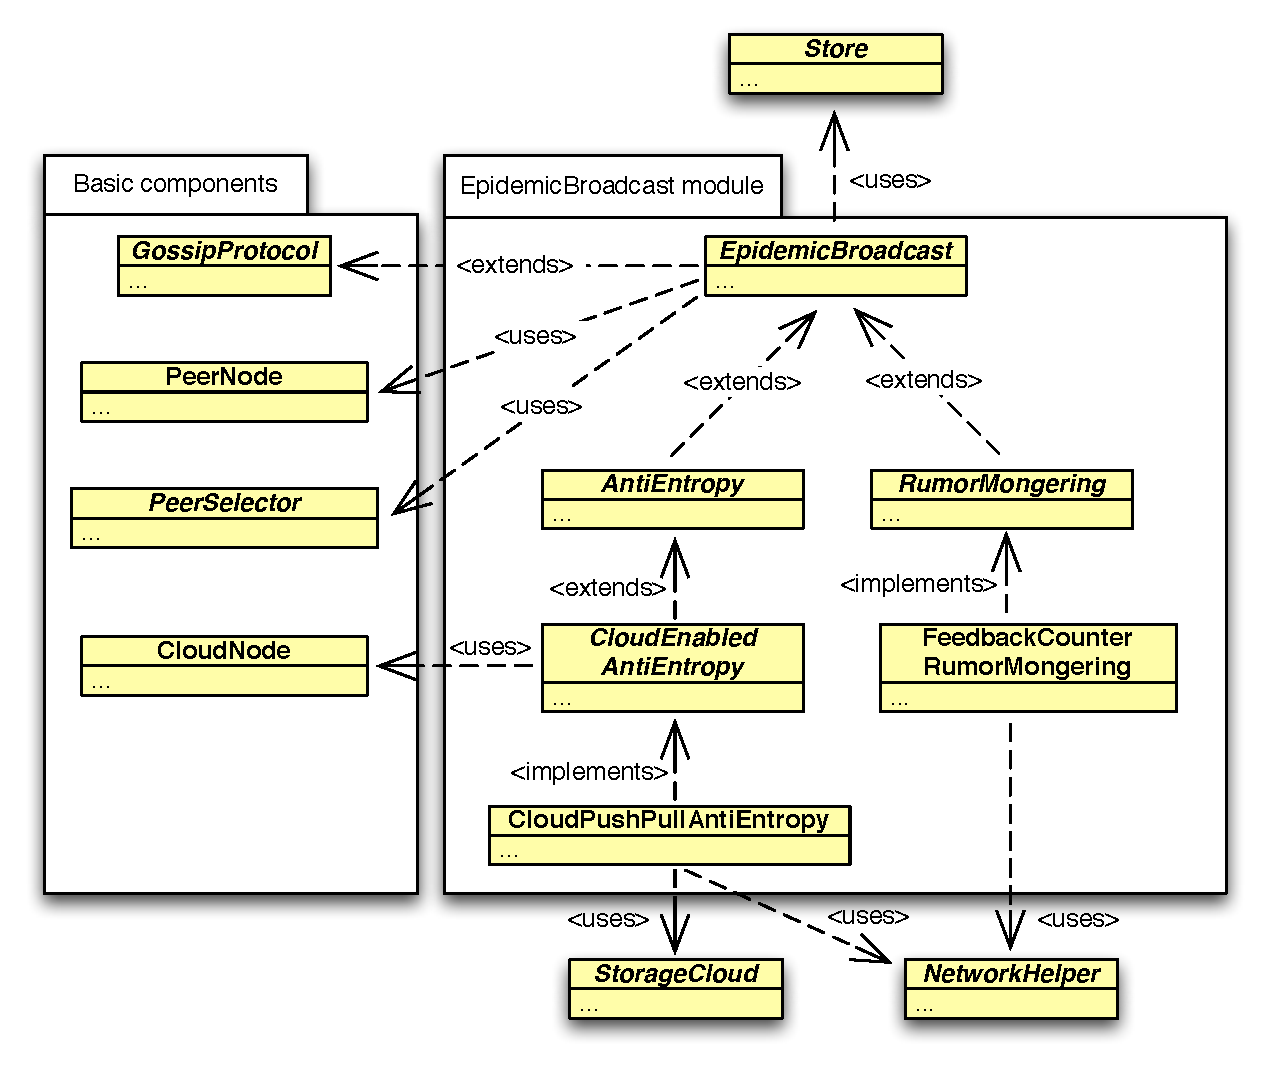
\includegraphics[width=\textwidth]{cloudypeer-epidemicbroadcast-relations.pdf}
  \caption{Relations between classes of the \textit{Epidemic
      broadcast} module}
  \label{fig:cloudypeer-epidemicbroadcast-relations}
\end{figure}

The structure of the module is for itself quite simple and intuitive as
can be noted analyzing the diagram shown in figure
\ref{fig:cloudypeer-epidemicbroadcast-relations}. By taking into
account the picture as a whole however it can be note that the module
display a strong dependence factor. Indeed here it is possible to see how
the \api infrastructure thus far defined comes into play to simplify
the development of high-level protocols. By heavily relaying on the
other modules, the implementation of the two \epidemic broadcast
protocols result very simple and most importantly general.

Figure~\ref{fig:cloudypeer-epidemicbroadcast-class} shows the main
classes forming the module's architecture and details the exposed
methods. Once again most of the functionalities are inherited from
\texttt{GossipProtocol} and the remaining one should be already clear
from previous considerations; refer to the \javadoc for further details.

\begin{figure}[h]
  \hspace{-50pt}
  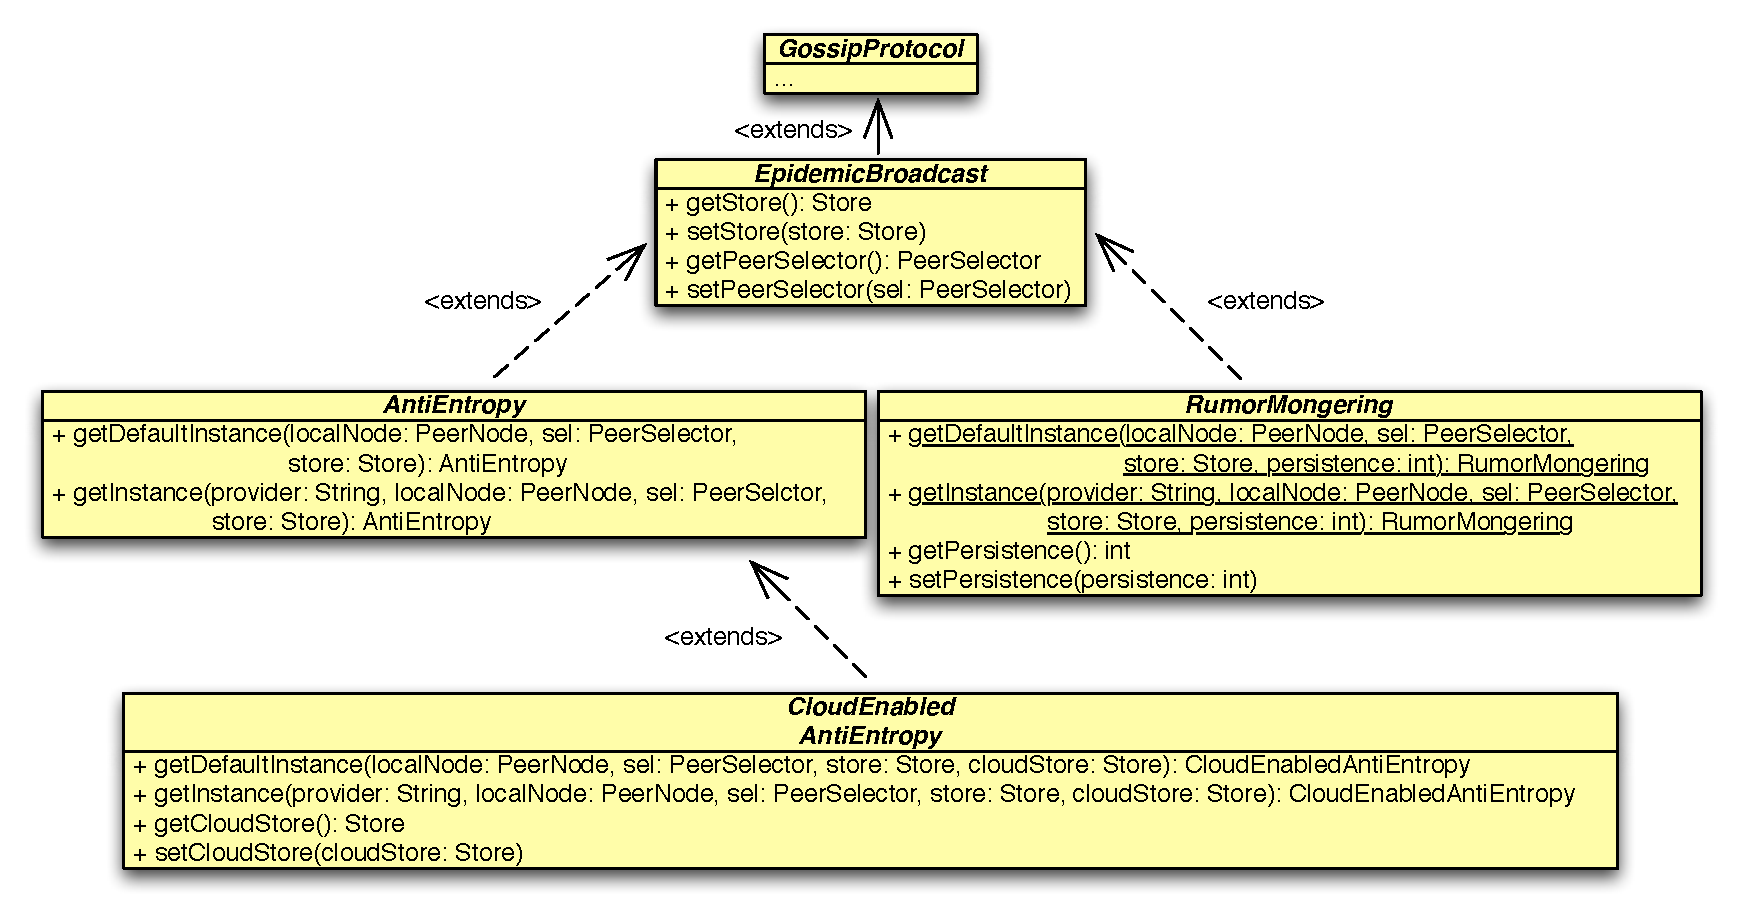
\includegraphics[width=1.3\textwidth]{cloudypeer-epidemicbroadcast-classdiagram.pdf}
  \caption{Details of the \textit{Epidemic broadcast} module \api}
  \label{fig:cloudypeer-epidemicbroadcast-class}
\end{figure}

At the current state the framework provides two built-in protocol
implementations: \texttt{CloudPushPullAntiEntropy} and
\texttt{FeedbackCounterRumorMongering}. As their names suggest, the
former uses a \PUSHPULL\ strategy and displays support for the \cloud while
the latter implements a standard \rumormongering algorithm with peer
feedback and termination based on counter.
Even though the implementations follow closely what has been stated in
section~\ref{sec:epidemicbroadcast}, in the following paragraphs are
explained in detail the executed procedures with the intent of
clarifying the interactions with the various \cloudypeer components.

\begin{figure}[h]
  \centering
  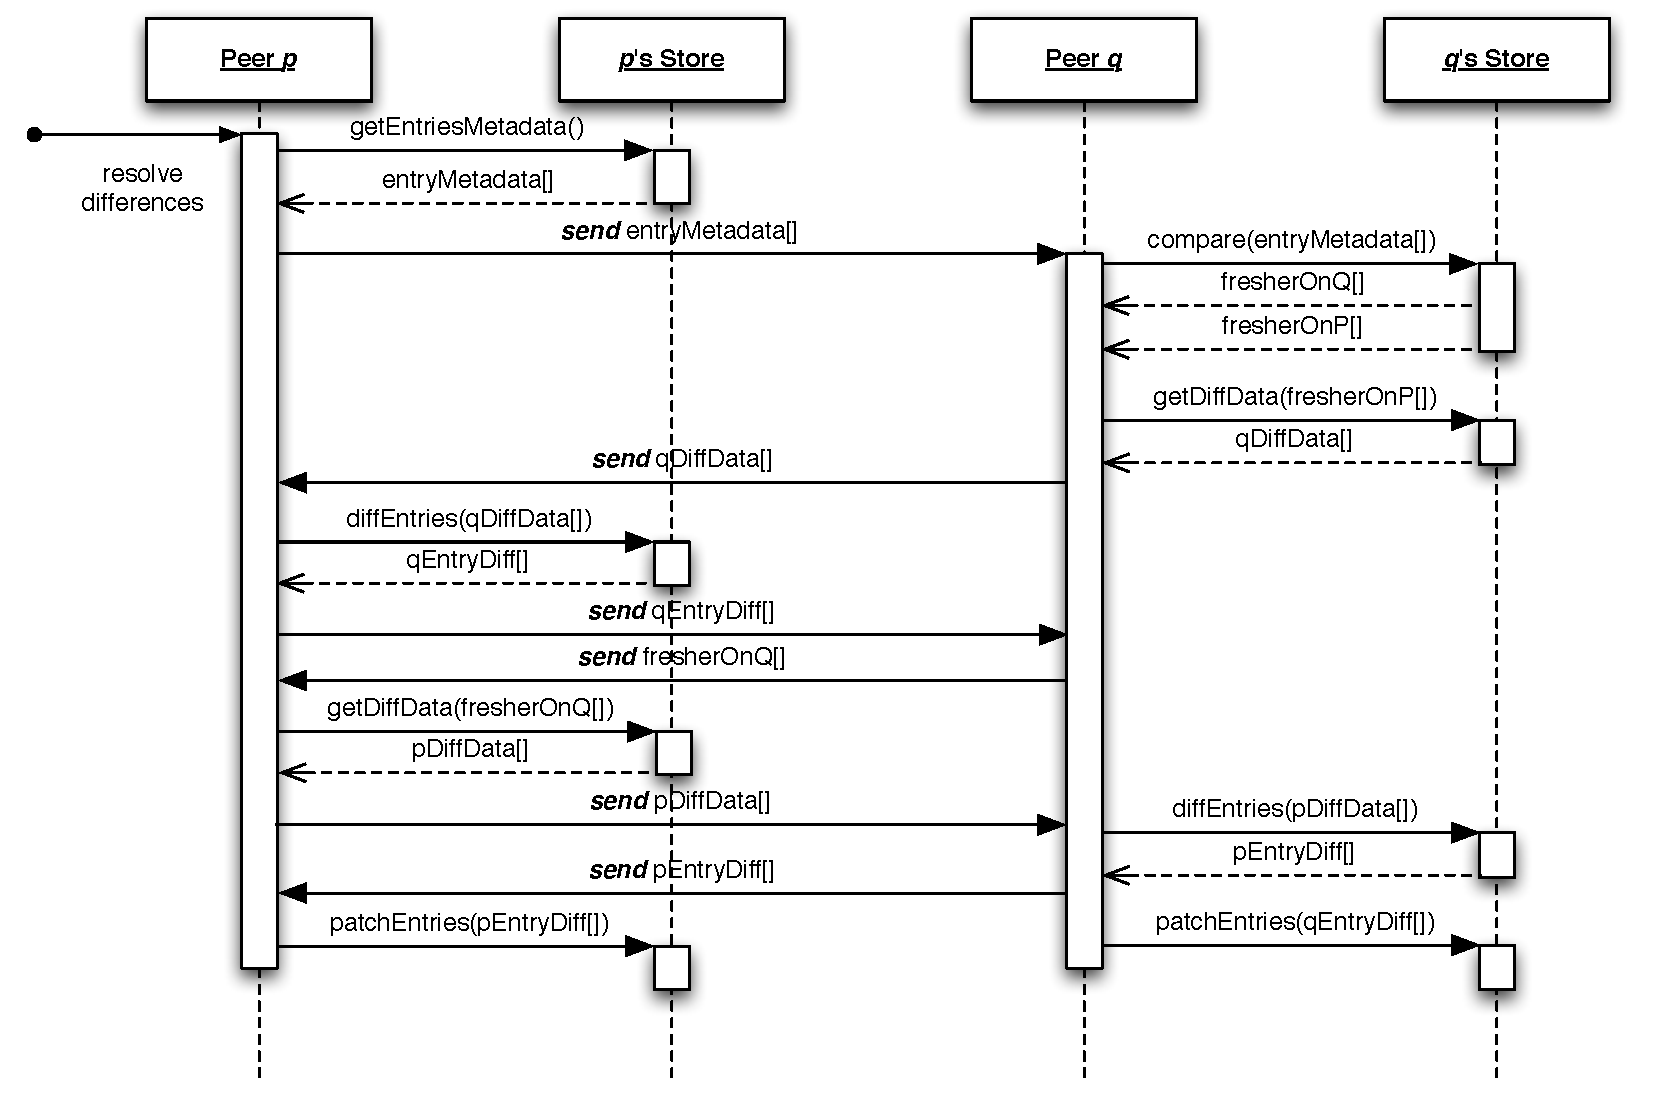
\includegraphics[width=\textwidth]{cloudypeer-antientropy-peer.pdf}
  \caption{Sequence diagram of an \antientropy\ cycle involving a remote
    peer (\PUSHPULL\ strategy)}
  \label{fig:cloudypeer-sequence-antientropy-peer}
\end{figure}

Figure~\ref{fig:cloudypeer-sequence-antientropy-peer} shows an
\antientropy cycle between two peers. As a first operation the
initiating peer $p$ queries its \texttt{Store} for the entries'
metadata. These are sent, using the \networkhelper, to the remote
peer $q$ which delegates to its \texttt{Store} instance the job of
analyze them. As a result of this operation, $q$ obtains two lists:
one for the entry to be pulled and one for the entry to be pushed.
At this point $q$ produces and sends the data which  $p$ uses to generate
the \textit{diff} information needed to patch $q$'s \texttt{Store}. The
same process is subsequently performed with switched roles concluding
the messages exchange between the two peers which at this point can
update their respective \texttt{Store} and conclude the execution.

\begin{figure}[h]
  \centering
  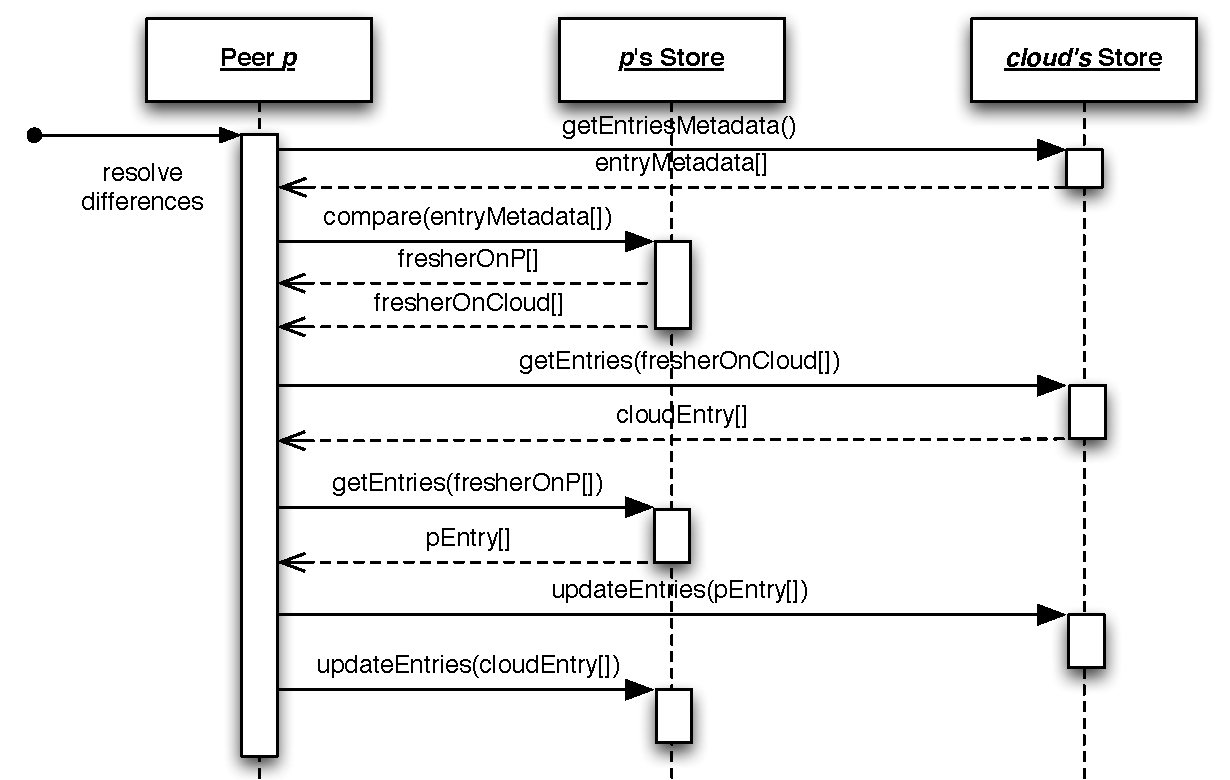
\includegraphics[width=\textwidth]{cloudypeer-antientropy-cloud.pdf}
  \caption{Sequence diagram of an \antientropy\ cycle involving the
    \cloud\ (\PUSHPULL\ strategy)}
  \label{fig:cloudypeer-sequence-antientropy-cloud}
\end{figure}

\ \\
\noindent Figure~\ref{fig:cloudypeer-sequence-antientropy-cloud} displays the
actions executed when an \antientropy cycle involves the \cloud. As
can be seen all the computation is performed by the initiating peer
which orchestrates the entire exchange. The followed steps are similar
to the ones described for the previous case, however the passive
nature of the \cloud causes a major difference: the whole data is
transferred in both the direction. This fact means that data exchanged
with the \cloud may display much higher bandwidth costs with respect
to the same exchange between two peers. Fortunately, as it is
discussed later, this problem does not have an high impact on the
overall cost.

\ \\
\noindent The last diagram, shown in
figure~\ref{fig:cloudypeer-sequence-rumormongering}, illustrate the
behavior of the \rumormongering implementation. Here the similarities
with the first case are much more evident. Indeed the higher half of the
diagram display exactly the same operation. The few differences are
represented by the fact that updates only flow in one direction and
more importantly that the triggering factor is not the firing of a
timer but instead the notification by the \texttt{Store} which a new
update is available.

\begin{figure}[H]
  \centering
  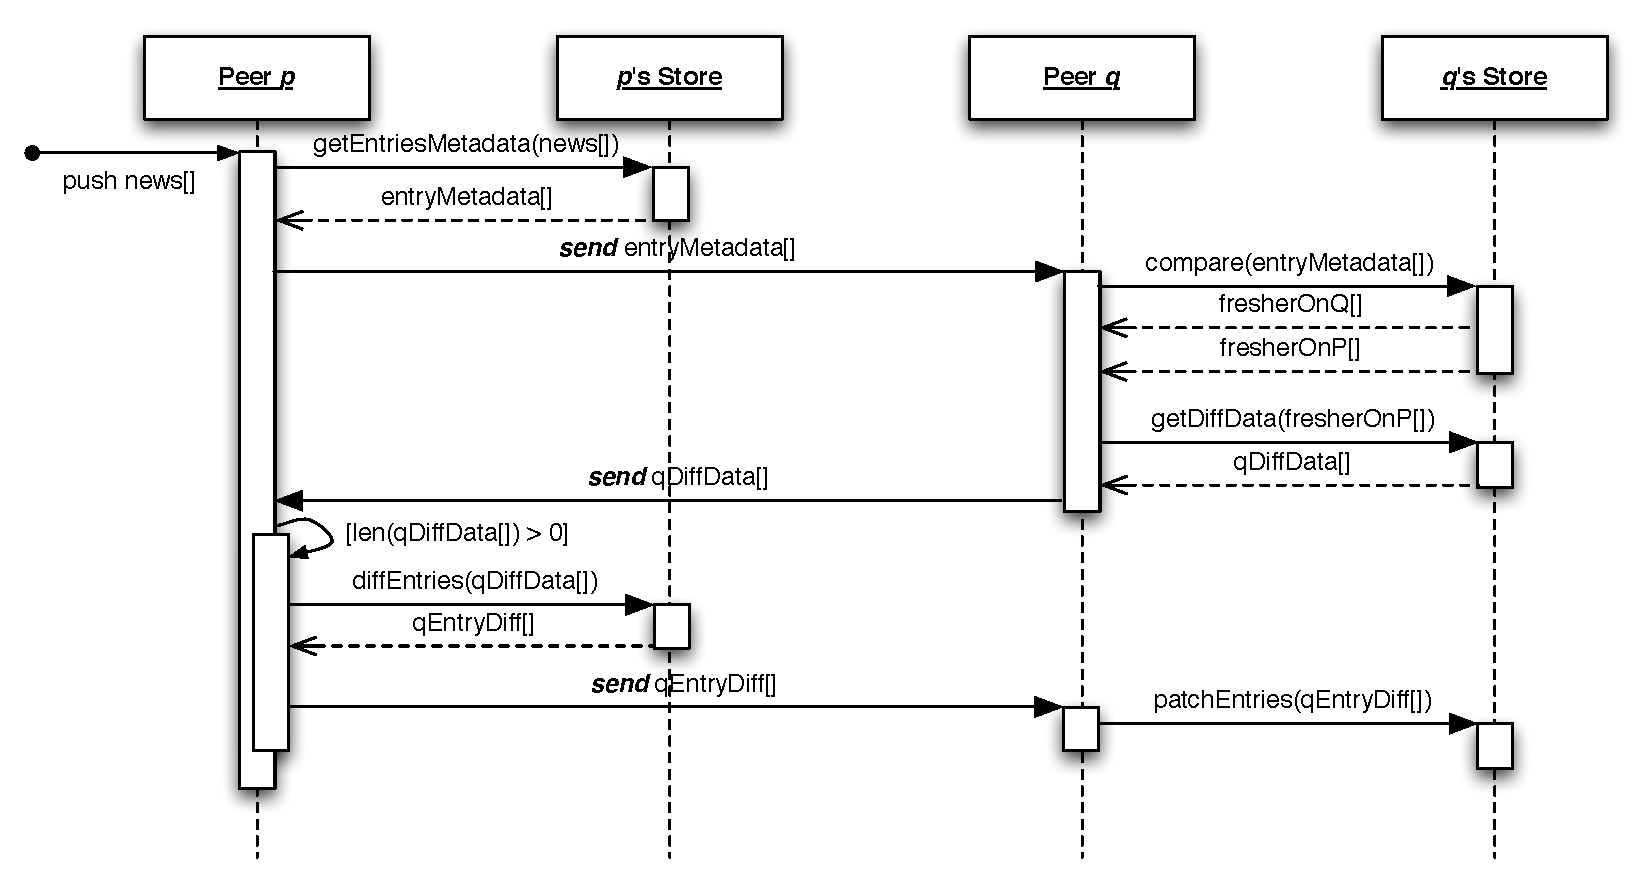
\includegraphics[width=\textwidth]{cloudypeer-rumormongering.pdf}
  \caption{Sequence diagram of a \rumormongering\ cycle}
  \label{fig:cloudypeer-sequence-rumormongering}
\end{figure}

\clearpage
\section{Building and using the framework}
To conclude the analysis of the framework, in this section is
explained how \cloudypeer can be compiled and used by developers to
write their \ptop applications.

As for the other library developed during the course of this thesis,
the code is available via a \github repository~\cite{cloudypeer-repo}
with the last version available at the time of this writing tagged
with \thesistag.

The distribution already contains all the \textit{Java} dependencies,
including \jgrapes. Thus to build the framework it is sufficient to invoke the
\textit{dist} target of the \textit{ant} build file. This operation will
generate a directory named \textsf{dist/} containing the \textit{jar}
files of \cloudypeer and all the other dependencies.

At this point the framework can be used by simply adding the various
\textit{jars} to the \textit{Java classpath}. To successfully use the
\jgrapes based \peersampling protocol implementation however, the
\textit{Java} property ``java.library.path'' must be configured
to include the directory containing all the relative native
libraries. Such a directory is produced during the building process of
\jgrapes under the name \textsf{dist}.

The listing available in figure~\ref{lst:cloudypeer-example-app}
provide a fully working, even if minimal, application based on \cloudypeer.
As can be noted the amount of code needed by the developer to setup
the \cloudcast infrastructure is really small: skipping comments,
blank lines and variable declarations only $19$ operations are
required.

This example only serves the role of demonstrating the convenience
offered by the framework, more elaborated examples are available in
the codebase of \cloudypeer under the \textit{test} package.

\begin{figure}[H]
  \lstinputlisting[language=Java,basicstyle=\footnotesize,numberstyle=\footnotesize,numbers=left,frame=leftline]{code/cloudypeer-example.java}
  \hspace{-100pt}
  \caption{Skeleton of a simple application exploiting \cloudypeer}
  \label{lst:cloudypeer-example-app}
\end{figure}

\section{Evaluation}
In this section are proposed some results showing the
effectiveness of the framework in terms of \textit{news}
distribution.

Let's start by analyzing the delays in the delivery of \textit{news}
considering a dynamic scenario. Figure
\ref{fig:cloudypeer-oscillating-delays} match plot
\ref{fig:cloudcast-sim-oscillating-delays} which is re-proposed here
for convenience. Due to lack of resources it has not been possible to
perform the test under exactly the same conditions: the maximal network
size had to be limited to $170$ nodes instead of $500$. However all
the other parameters have been maintained: the experiment has lasted 2
days with a new
\textit{news} added each four hours. The \antientropy and
\rumormongering protocols have been configured with a period of
respectively $10$ and $1$ seconds.

As can be seen the delays obtained by the \cloudypeer implementation
are slightly smaller with respect to the ones recorded during the
simulation.
This variation can be partially attributed to
the different network sizes, however it is our opinion that the
improved result is achieved mostly thanks to the more elaborated
\rumormongering protocol which, exploiting peer's feedback, is more
effective in quickly diffusing updates.

\begin{figure}[H]
  \centering
  \subfloat[][\cloudypeer experiment]{
    \hspace{-70pt}
    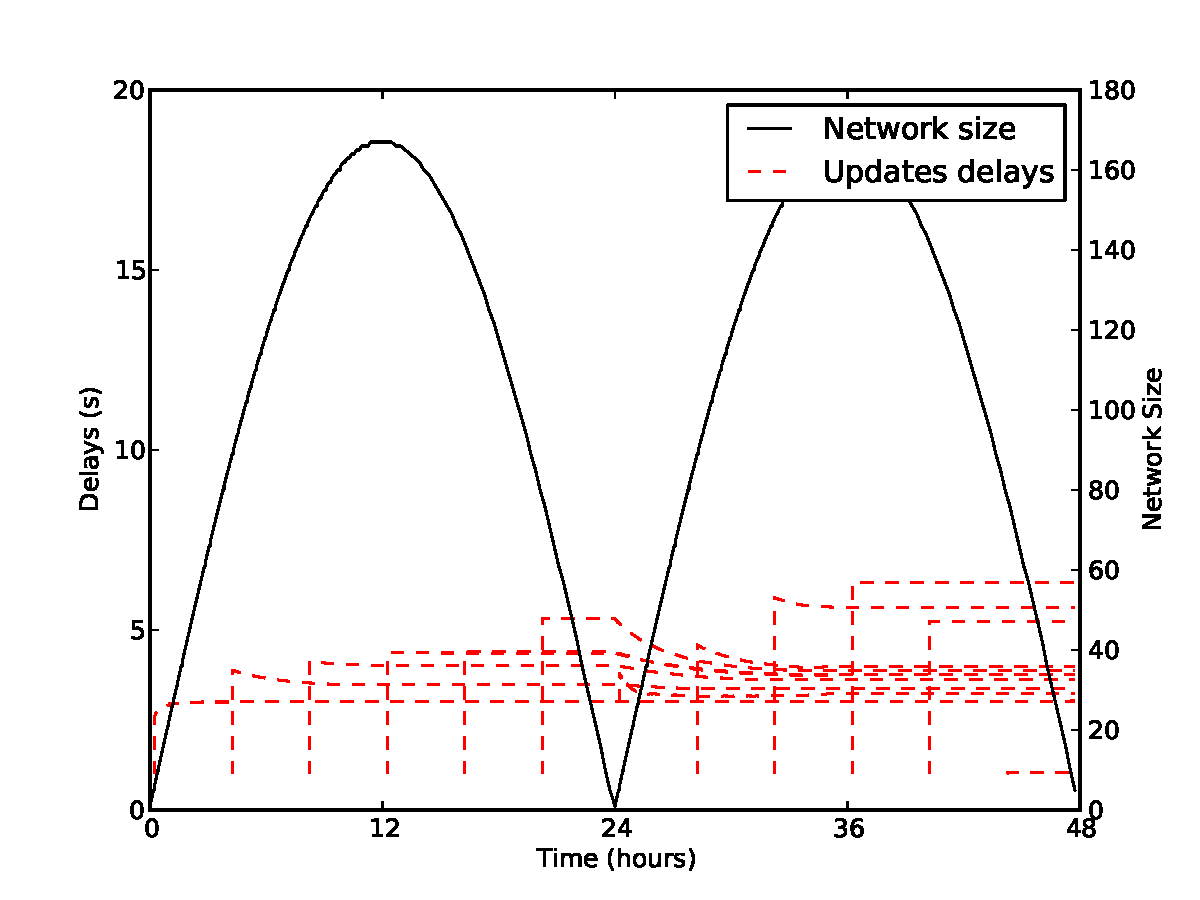
\includegraphics[width=240pt]{cloudypeer-oscillating-delays.pdf}
    \label{fig:cloudypeer-oscillating-delays}
  }
  \subfloat[][Simulated \cloudcast experiment]{
    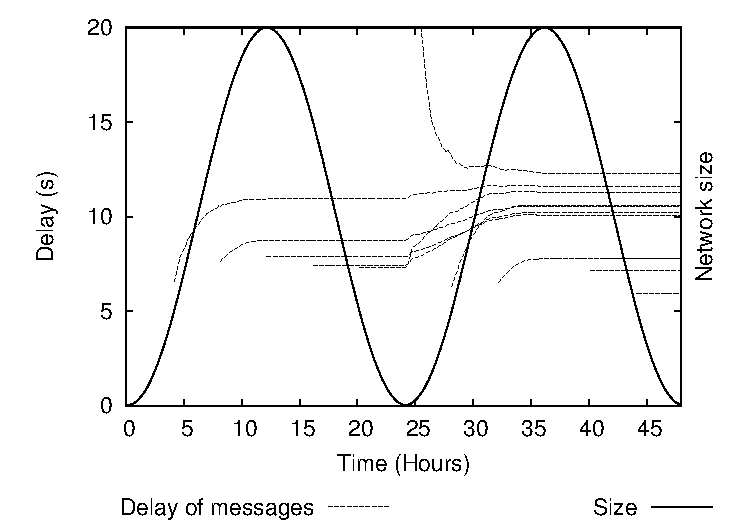
\includegraphics[width=240pt]{cloudcast-sim-oscillating-delays.pdf}
  }
  \caption{Progressive delays in message diffusion in a dynamic scenario}
  \label{fig:cloudcast-globa-delay}
\end{figure}

Another interesting measure of evaluation is represented by the
traffic generated by the system. In this case we are not interested
in the actual number of bytes exchanged but instead we focused our
analysis on the number of times each node \textit{pushed} some
data. The rationale behind this reasoning is that the framework allows
to easily change the actual network implementation and \textit{diff}
strategy, hence a measure influenced by these components would not be
of much value.

The experiments have been setup to employ a network
which linearly grows up to a target size and exchanges \textit{news}
generated with a $5$ minutes period for a total duration of one hour.
Each configuration has been iterated $10$ times and the displayed
values represent the aggregated statistics.
Due to lack of time and resources it has not been possible to
experiment on networks with a more significative size; future works may
fill this gap by providing more exhaustive results.

The data about node's exchanges shown in table~\ref{tbl:pushed-news}
displays a predictable scenario: the majority of the
work is carried out by the \rumormongering protocol while \antientropy
has a much smaller impact. Of more interest is the data regarding the
number of news that have been pushed by \cloud, presented in
table~\ref{tbl:cloud-news}: the mean values are really small compared
to the total amount of updates transferred during the whole
experiment. In particular it can be noted how the contribution of the
\cloud never surpasses the $2\%$ of the total. This demonstrates once
again the effectiveness of the \cloudcast approach and at the same
time proves the correctness of the implementation.

\begin{table}[h!]
  \centering
  \begin{tabular}{|c|c|c|c|c|c|c|c|c|}
  \hline
  Size & Protocol & Avg & Var & Min & Q1 & Q2 & Q3 & Max\\
  \hline
  \hline

  \multirow{2}{*}{32} &
        \antientropy & 3.32 & 5.45 & 0 & 1 & 3 & 5 & 11 \\

       &\rumormongering & 8.57  & 9.89 & 1 & 6 & 8 & 11 & 16\\

  \hline
  \multirow{2}{*}{64} &
        \antientropy & 2.87 & 4.32 & 0 & 1 & 3 & 4 & 10\\

      & \rumormongering & 9.08 & 10.93 & 2 & 7 & 9 & 11 & 21\\

  \hline
  \multirow{2}{*}{128} &
        \antientropy & 2.52 & 4.15 & 0 & 1 & 2 & 4 & 14\\

      & \rumormongering & 9.35 & 13.28 & 1 & 7 & 9 & 12 & 22 \\

  \hline
  \multirow{2}{*}{160} &
        \antientropy & 2.80 & 5.66 & 0 & 1 & 2 & 4 & 16\\

      & \rumormongering & 9.027 & 13.54 & 1 & 6 & 9 & 11 & 24 \\
  \hline
  \end{tabular}
  \caption{Statistic on the \textit{news} pushed by the \epidemic
    broadcast protocols}
  \label{tbl:pushed-news}
\end{table}

\begin{table}[h!]
  \hspace{-30pt}
  \begin{tabular}{|c|c|c|c|c|c|c|c|c|c|}
  \hline
  Size & Updates \# & Cloud \% & Cloud Avg & Cloud Var & Min & Q1 & Q2 & Q3 & Max\\
  \hline
  \hline
  32 & 384 & 1.45\%  & 5.59 & 5.44 & 2 & 3 & 6 & 8 & 8 \\
  64 & 768 & 0.73\% & 5.79 & 7.76 & 3 & 3 & 5 & 9 & 10 \\
  128 & 1536 & 1.2\% & 19.19 & 29.76 & 11 & 13 & 21 & 24.5 & 26\\
  160 & 1920 & 1.72\% &33.03 & 44.12 & 26 & 27 & 30 & 40.5 & 44 \\
  \hline
  \end{tabular}
  \caption{Statistic on the \textit{news} obtained via the \cloud}
  \label{tbl:cloud-news}
\end{table}
